\documentclass{ximera}
%% handout
%% nohints
%% space
%% newpage
%% numbers

%% You can put user macros here
%% However, you cannot make new environments

\graphicspath{{./}{secondExample/}}

\usepackage{tikz}
\usepackage{tkz-euclide}
\usetkzobj{all}

\tikzstyle geometryDiagrams=[ultra thick,color=blue!50!black]
 %% we can turn off input when making a master document

\prerequisites{none}
\outcomes{ximeraLatex}

\title{Visualizing Functions}

\begin{document}
\begin{abstract}
We learn three methods for presenting functions: graphing, tables, and formulas.
\end{abstract}
\maketitle

There are three nice methods for presenting a function. We can draw its graph in the plane, create a table, and/or write a formula.

For example, Let $A(x)$ be the the area of the triangle below.
\[
\begin{tikzpicture}
\draw (0,0) --node[below]{$x$} (2,0) -- (0,2) --node[left]{$x$} (0,0) rectangle (.2,.2);
\end{tikzpicture}
\]
\begin{itemize}
\item We can represent $A(x)$ as a table.
\[
\begin{tabular}{cccccccc}
$x$ & $0$ & $1$ & $2$ & $3$ & $4$ & $5$ & $6$\\ \hline
$A(x)$ & $0$ & $.5$ & $2$ & $4.5$ & $8$ & $12.5$ & $18$
\end{tabular}
\]
\item
We can represent $A(x)$ as a formula. The area of a triangle is one half base times height, so $A(x)=\frac{1}{2}x^2$.
\item We can draw a graph of $y=A(x)$.
\begin{image}
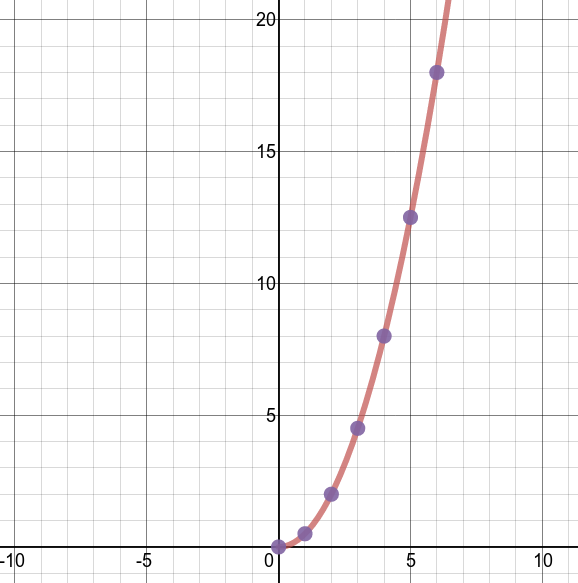
\includegraphics[width=8cm]{IntroToFunctions/Functions/TriangleArea.png}
\end{image}
\end{itemize}

All three methods of presenting the function are useful, though some circumstances might make one method more useful than another. The good news is that we will be using a tool to help us obtain these various representations of functions. Watch the video below to learn how to obtain a graph and a table from a function.



\end{document}